\documentclass[final]{fhnwreport}       %[mode] = draft or final
                                        %{class} = fhnwreport, article, 
                                        %          report, book, beamer, standalone
%%---Main Packages-----------------------------------------------------------------------
\usepackage[english, ngerman]{babel}	%Mul­tilin­gual sup­port for LaTeX
\usepackage[T1]{fontenc}				%Stan­dard pack­age for se­lect­ing font en­cod­ings
\usepackage[utf8]{inputenc}				%Ac­cept dif­fer­ent in­put en­cod­ings
\usepackage{lmodern}                    %The newer Font-Set
\usepackage{textcomp}					%LaTeX sup­port for the Text Com­pan­ion fonts
\usepackage{graphicx} 					%En­hanced sup­port for graph­ics
\usepackage{float}						%Im­proved in­ter­face for float­ing ob­jects
\usepackage{ifdraft}                    %Let you check if the doc is in draft mode

%%---Useful Packages---------------------------------------------------------------------
\usepackage[pdftex,dvipsnames,table]{xcolor}  %Driver-in­de­pen­dent color ex­ten­sions for LaTeX
\usepackage{csquotes}                   %Simpler quoting with \enquote{}
\usepackage{siunitx} 					%A com­pre­hen­sive (SI) units pack­age
\usepackage{listings}					%Type­set source code list­ings us­ing LaTeX
\usepackage[bottom]{footmisc}			%A range of foot­note op­tions
\usepackage{footnote}					%Im­prove on LaTeX's foot­note han­dling
\usepackage{verbatim}					%Reim­ple­men­ta­tion of and ex­ten­sions to LaTeX ver­ba­tim
\usepackage[textsize=footnotesize]{todonotes} %Mark­ing things to do in a LaTeX doc­u­ment
\usepackage{booktabs}
\usepackage{lscape}
\usepackage{blindtext}
\usepackage{wrapfig}

%%---Tikz Packages-----------------------------------------------------------------------
\usepackage{standalone}
\usepackage{tikz}
\usepackage{circuitikz}
\usetikzlibrary{arrows}
\usetikzlibrary{calc}
\usetikzlibrary{intersections}

%%---Math Packages-----------------------------------------------------------------------
\usepackage{amsmath}					%AMS math­e­mat­i­cal fa­cil­i­ties for LaTeX
%\usepackage{amssymb}					%Type­set­ting symbols (AMS style)
%\usepackage{array}						%Ex­tend­ing the ar­ray and tab­u­lar en­vi­ron­ments
%\usepackage{amsthm}					%Type­set­ting the­o­rems (AMS style)

%%---Table Packages----------------------------------------------------------------------
\usepackage{tabularx}					%Tab­u­lars with ad­justable-width columns
%\usepackage{longtable}
\usepackage{multirow}					%Create tab­u­lar cells span­ning mul­ti­ple rows
\usepackage{multicol}					%In­ter­mix sin­gle and mul­ti­ple columns

%%---PDF / Figure Packages---------------------------------------------------------------
\usepackage{pdfpages}					%In­clude PDF doc­u­ments in LaTeX
\usepackage{pdflscape}					%Make land­scape pages dis­play as land­scape
\usepackage{subfig}					    %Fig­ures di­vided into sub­fig­ures

%%---Other Packages----------------------------------------------------------------------
%\usepackage{xargs}                     %De­fine com­mands with many op­tional ar­gu­ments

%%---Bibliography------------------------------------------------------------------------
\bibliographystyle{unsrt}

%%---Main Settings-----------------------------------------------------------------------
\graphicspath{{./graphics/}}			%Defines the graphicspath
%\geometry{twoside=false}				    %twoside=false disables the "bookstyle"
\setlength{\marginparwidth}{2cm}
\overfullrule=5em						%Creates a black rule if text goes over the margins => debugging


%%---User Definitions--------------------------------------------------------------------
%%Tabel-Definitions: (requires \usepackage{tabularx})
\newcolumntype{L}[1]{>{\raggedright\arraybackslash}p{#1}}    %column-width and alignment
\newcolumntype{C}[1]{>{\centering\arraybackslash}p{#1}}
\newcolumntype{R}[1]{>{\raggedleft\arraybackslash}p{#1}}

%%---Optional Package Settings-----------------------------------------------------------
%Listings-Settings: (requires \usepackage{listings}) => Example with Matlab Code
\lstset{language=Matlab,%
    basicstyle=\footnotesize\ttfamily,
    breaklines=false,%
    morekeywords={switch, case, otherwise},
    keywordstyle=\color{Blue},%
    tabsize=2,
    %morekeywords=[2]{1}, keywordstyle=[2]{\color{black}},
    identifierstyle=\color{Black},%
    stringstyle=\color{Purple},
    commentstyle=\color{Green},%
    showstringspaces=false,%without this there will be a symbol in the places where there is a space
    numbers=left,%
    numberstyle={\tiny \color{black}},% size of the numbers
    numbersep=9pt, % this defines how far the numbers are from the text
    %emph=[1]{word1, word2,...},emphstyle=[1]\color{red}
}										                %loads all packages, definitions and settings												
\title{\Huge{\textbf{Pflichtenheft}}\\}          %Project Title
\author{\huge{Wetterstation mit Solar Energie}}          %Document Type => Technical Report, ...
\date{Windisch, \today}             %Place and Date


\begin{document}

%%---TITLEPAGE---------------------------------------------------------------------------
\selectlanguage{ngerman}                %ngerman or english
\maketitle
%\vspace*{-1cm}
\vspace*{-0.5cm}						    %compensates the space after the date line.
\vfill
\begin{figure}[H]
\centering
%\includegraphics[width=\linewidth]{Titelbild.jpg}
\end{figure}
\vfill

{
\renewcommand\arraystretch{2}
\begin{center}
\begin{tabular}{>{\bf}p{4cm} l}
Hochschule		&	Hochschule für Technik - FHNW\\
Studiengang		&	Elektro- und Informationstechnik\\
Auftraggeber	&	Prof. Dr. Taoufik Nouri\\
Experte			&	Patrick Strittmatter\\
Betreuer		&	Prof. Dr. Taoufik Nouri\\
Autoren		&	Mischa Knupfer, Andres Minder\\
Version			&	1.0 %Normally not used!
\end{tabular}
\end{center}
}

\clearpage
			
%%---ABSTRACT----------------------------------------------------------------------------
\selectlanguage{english}				%ngerman or english
\thispagestyle{empty}
\section*{Einleitung}
\todo{Die Einleitung sollte offensichtlich noch geschrieben werden.}
\section*{Auftragsbeschreibung}
Das Wetter spielt eine wichtige Rolle in der Agronomie. Aufgrund von Wetter- und Klimadaten können optimale Standorte für Pflanzen eruiert und Massnahmen zu deren Schutz getroffen werden. Hiesige Bauern besitzen den Luxus von guten Wettervorhersagen und Klimadaten dank dem Bundesamt für Meteorologie und Klimatologie (MeteoSchweiz). Dieser Luxus ist in anderen Ländern noch nicht gegeben. Prof. Dr. Nouri Taoufik ist aufgefallen, dass in tropischen Gegenden wie Südamerika oder teile Afrikas dieser Luxus ebenso fehlt. \\[0.5cm]
Aus diesem Grund soll eine kostengünstige, erweiterbare und mobile Wetterstation gebaut werden, welche diese Bauern unterstützt. Diese Wetterstation soll die Regenmenge, die Windstärke, die Lufttemperatur und die Sonnenstunden messen können. Ausserdem soll die Wetterstation mittels Photovoltaik unterstützt werden, und erhobene Daten via SMS abrufbar sein. \\[0.5cm]
In einem ersten Projekt wurde die Sensorik zur Messung der Lufttemperatur, Luftfeuchtigkeit, Luftdruck, Regenmenge, Windstärke und Windrichtung implementiert, jedoch nicht verifiziert. Ausserdem wurde eine RTC implementiert, welche Zeitstempel liefert um die erhobenen Daten zu datieren. Auf einer $\mu$SD-Karte können Daten gespeichert und über eine serielle Schnittstelle ausgegeben werden. Das ganze wird über eine MCU gesteuert. \\[0.5cm]
Im Nachfolgenden Dokument werden unter anderem die Ziele dieses Projekts definiert, sowie das Gesamtkonzept näher erläutert. \todo[inline]{Auftragsbeschreibung kontrollieren und Verbesserungsvorschläge machen.}

%\begin{abstract}

\end{abstract}	

%%---TABLE OF CONTENTS-------------------------------------------------------------------
\pagenumbering{Roman}		
\selectlanguage{ngerman}				%ngerman or english
\tableofcontents
\clearpage

%%---TEXT--------------------------------------------------------------------------------
\pagenumbering{arabic}
\cleardoublepage

\begin{center}
\vspace*{4cm}
\section*{\Huge{Technischer Teil}}
\addcontentsline{toc}{section}{Technischer Teil}
\end{center}
\cleardoublepage
\vspace*{4cm}
\thispagestyle{empty}
\begin{center}
	\section{Organisatorischer Teil}
\end{center}
\todo{Falls möglich, hier die Schriftgrösse ändern. Sieht sonst etwas spärlich aus.}
\newpage

\begin{landscape}
\subsection{Ziele}
Die Tabelle \ref{tab:ZieleP6} zeigt die diskreten Ziele dieses Projektes. Darin enthalten sind die jeweiligen zu erreichenden Muss-, Nicht- und Wunschziele mit ihren quantifizierten Spezifikationen.\\
\begin{table}[htbp]
  \centering
  \renewcommand{\arraystretch}{1.1} %Angepasst da sonst neue Seite
  \caption{Ziele}
    \begin{tabular}{l|l|l|r|r}
          & \textbf{Ziel} & \multicolumn{1}{l|}{\textbf{Spezifikation}} & \multicolumn{1}{l|}{\textbf{Genauigkeit}} & \multicolumn{1}{l}{\textbf{Einheit}} \\
    \toprule
    \multicolumn{1}{l}{\textbf{Mussziele}} & \multicolumn{4}{r}{} \\
    \toprule
  \multirow{3}{*}{Speisung} & Akkulaufzeit & \multicolumn{1}{r|}{$\geq$\,100} &   & h \\
    \cline{2-5}  & Mittels DC-Ladekabel ladbar &      5.5 / 2.1mm DC-Stecker &       &  \\
	\cline{2-5}           & Photovoltaik &    \multicolumn{1}{r|}{1}   &       & Akkuladungen/Tag \\
    \hline
  \multirow{2}{*}{Kommunikationsmodule} & GPS-Modul Standortupdate   &  \multicolumn{1}{r|}{<\,5}  &       & Minuten \\
	\cline{2-5}          & GSM-Modul  & SMS: Senden und Empfangen &       &  \\
\hline
Sensoren & Sonnenstunden (Lichtstromdichte) & \multicolumn{1}{r|}{0.1 - 90'000} & & lx \\
    \bottomrule
    \multicolumn{1}{l}{\textbf{Nichtziele}} & \multicolumn{4}{r}{} \\
    \toprule
     Sensoren aus Projekt 5& Keine Neukonzeption &  &  &  \\
     \hline
     Wartungsfreiheit & Wartungsfenster & \multicolumn{1}{r|}{>7} &  & Tage \\
    \bottomrule
    \multicolumn{1}{l}{\textbf{Wunschziele}} & \multicolumn{4}{r}{} \\
    \toprule
    Kommunikationsmodule & Einbindung in IoT &       Bluetooth || WLAN &       &  \\
    \hline
    \multirow{2}{*}{Speisung} & Akku leicht austauschbar &       &       &  \\
\cline{2-5}  & Mittels USB ladbar & USB 2.0 (Mini-B || Micro-B) &       &  \\

    \bottomrule
    \end{tabular}%
  \label{tab:ZieleP6}%
\end{table}%

Tabelle \ref{tab:ZieleP6} zeigt die Muss-, Nicht- und Wunschziele des Projekts auf. Die Akkulaufzeit und das Laden mittels DC-Ladekabel sind spezifiziert. Ausserdem wird ein volles Aufladen des Akkus innerhalb eines Tages via Photovoltaik als Ziel gesetzt. Dabei wird von der maximal möglichen Leistung der Photovoltaik ausgegangen, bei einer optimalen Sonneneinstrahlung von 10 Stunden. Das Update des Standorts wird spätestens alle 5 Minuten erfolgen und das Empfangen und Senden von SMS wird ebenfalls möglich sein. Nicht Ziel des Projekts ist es, die in einem vorhergehenden Projekt entworfene Sensoren neu zu konzipieren, sowie die mobile Wetterstation komplett Wartungsfrei zu machen. Eine wöchentliche Wartung ($\leq$ 7 Tage) wird als vertretbar bis notwendig erachtet. Als Wunschziel folgt die Einbindung der mobilen Wetterstation in das \textit{IoT}, ein leicht austauschbarer Akku, sowie die Möglichkeit, den Akku in der mobilen Wetterstation via USB-Kabel zu laden.

\end{landscape}

\section{Kommunikation}
Die Kommunikation erfolgt grundsätzlich per E-Mail, ausser für Notfälle. Dafür sind die Telefonnummern noch zusätzlich in diesem Dokument hinterlegt (siehe Tabelle \ref{tab:kontaktinformationen}). 

% Table generated by Excel2LaTeX from sheet 'Tabelle1'
\begin{table}[htbp]
  \centering
  \small
  \caption{Kontaktinformationen}
  \label{tab:kontaktinformationen}
    \begin{tabular}{l|l|l|l}
    \textbf{Projektinstanz} & \textbf{Name} & \textbf{E-Mail} & \textbf{Telefon} \\
    \toprule
    Auftraggeber/ & \multirow{2}[2]{*}{Prof. Dr. Taoufik Nouri} & \multirow{2}[2]{*}{\textcolor[rgb]{ .02,  .388,  .757}{taoufik.nouri@fhnw.ch}} & \multirow{2}[2]{*}{+41 79 218 38 55} \\
    Projektbetreuer &       &       &  \\
    \hline
    Projektteam & Mischa Knupfer & \textcolor[rgb]{ .02,  .388,  .757}{mischa.knupfer@students.fhnw.ch} & +41 78 761 83 73 \\
    \hline
    Projektteam & Andres Minder & \textcolor[rgb]{ .02,  .388,  .757}{andres.minder@students.fhnw.ch} & +41 79 810 82 13 \\
    \end{tabular}%
  \label{tab:addlabel}%
\end{table}%

\vspace{0.5cm}

Im Verlaufe dieses Projektes wird alle zwei Wochen eine Sitzung mit Herrn Prof. Dr. Taoufik Nouri und dem Projektteam abgehalten. Darin werden aktuelle Angelegenheiten diskutiert und jegliche pendente Themen angesprochen. Für aufgetretene Probleme wird konstruktiv nach Lösungen für das weitere Vorgehen gesucht. 

\vspace{0.5cm}

Die Sitzungseinladungen sind vom Projektteam aus zu verschicken, sowie auch die Sitzungen zu protokollieren. Jedes Protokoll wird innerhalb einer Woche nach der Sitzung per E-Mail vom Projektteam aus an alle Instanzen des Projektes gemäß Tabelle \ref{tab:kontaktinformationen} mit einer Aktionsliste\footnote{eine Liste mit Angaben, wer was in welchem Zeitraum zu erledigen hat} verschickt. Im darauffolgenden Protokoll wird die Annahme aller Instanzen dokumentiert.

\section{Risikoanalyse}
In einem Projekt können immer wieder Probleme auftreten. In diesem Kapitel wird sich mit diesem Thema auseinandergesetzt und gezeigt, mit welchen Methoden auf die unterschiedlichen Eventualitäten reagiert werden kann.
Nachfolgend sind mögliche Risiken tabellarisch aufgelistet, sowie Maßnahmen um diese zu vermindern.\\
% Table generated by Excel2LaTeX from sheet 'Tabelle1'
\begin{table}[htbp]
  \centering
  \caption{Risiken und Massnahmen}
    \begin{tabular}{|r|r|l|l|}
    \toprule
    \multicolumn{1}{|l}{\textbf{Risiken}} & \multicolumn{1}{r}{} &       & \textbf{Massnahmen} \\
    \hline
    \multicolumn{1}{|l|}{Nr.} & \multicolumn{1}{l|}{Kategorien} & Identifikation &  \\
    \hline
    1     & \multicolumn{1}{l|}{Student} & Ausfall wegen Krankheit & Keine spezielle Massnahme \\
\cline{1-1}\cline{3-4}    2     &       & Studiumsabbruch & Niemand hat dies vor \\
\cline{1-1}\cline{3-4}    3     &       & Konflikte im Team & Klare Kommunikation \\
\cline{1-1}\cline{3-4}    4     &       & Fachliche Überforderung & Hilfe suchen bei Dozenten \\
\cline{1-1}\cline{3-4}    5     &       & Terminliche Überforderung & Vorausschauende Zeitplanung \\
    \hline
    6     & \multicolumn{1}{l|}{Daten} & Notebook kaputt & Backup, Ersatznotebook \\
\cline{1-1}\cline{3-4}    7     &       & versehentliches löschen & Backup \\
    \hline
    8     & \multicolumn{1}{l|}{Sonstiges} & Teile werden nicht geliefert & Woanders bestellen/Express Lieferung\\
\cline{1-1}\cline{3-4}    9     &       & Kein eigener Arbeitsplatz & Platz im Studentenlabor \\
    \bottomrule
    \end{tabular}%
  \label{tab:RisikenUndMassnahmen}%
\end{table}%

Tabelle \ref{tab:RisikenUndMassnahmen} zeigt eine nummerierte Auflisten von möglichen Risiken und Massnahmen um diese zu vermindern. Eine Heat Map wird estellt, welche die Risiken nach Auswirkung und Eintrittswahrscheinlichkeit graphisch darstellt. Mit einem Pfeil wird die neue Position des Risikos mit greifender Massnahme angedeutet. So soll ein Überblick über mögliche Risiken und deren Potenzial gegeben werden.\\

\begin{figure}[h]
\centering
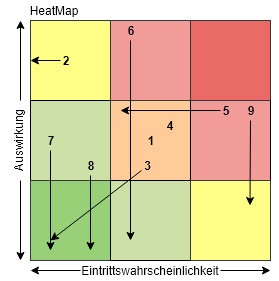
\includegraphics[scale=0.65]{graphics/HeatMap.PNG}
\caption{Heat Map}
\label{fig:HeatMap}
\end{figure}

Abbildung \ref{fig:HeatMap} gibt einen Überblick über mögliche Risiken und deren Potenzial, wobei die Nummern gemäss Tabelle \ref{tab:RisikenUndMassnahmen} definiert sind. Es ist ersichtlich, dass einige Massnahmen gewisse Risiken stark minimieren. Die grössten Risiken sind der Ausfall wegen Krankheit und fachliche sowie terminliche Überforderung. Auf diese Risiken soll während des Projekts speziell geachtet werden, um eine frühzeitige Erkennung zu gewährleisten.\\ 

\subsection{Budget}
%\todo[inline]{Es müssen die verwendeten Teile des P5 aufgeschrieben und deren Kosten aufgezeigt werden. Zusätzlich muss erwähnt werden, dass die Arbeit von uns Projektteilnehmern nicht inkludiert ist. Dazu gehören noch die allenfalls benötigten Bauteile. Auch wenn dies nur eine ungefähre Schätzung ist sollten diese Kosten vermerkt werden.}
Von Herrn Prof. Dr. Taoufik Nouri wurde kein ausdrücklich einzuhaltendes Budget vorgegeben, weshalb eine Budgetierung für die Entwicklung dieses Projekts nicht nötig ist. Zudem ist in dem im Anhang \ref{sec:aufgabenstellung} hinterlegten Dokument unter \textit{Bemerkungen} beschrieben, dass Anschaffungen von Hardware außerhalb der FHNW zuerst mit Herrn Prof. Dr. Taoufik Nouri besprochen werden muss. Somit bleibt es ihm vorbehalten, wann Bauteile zu hohe Kosten tragen.\\

\todo[inline]{Lesen und korrigieren/verbessern}
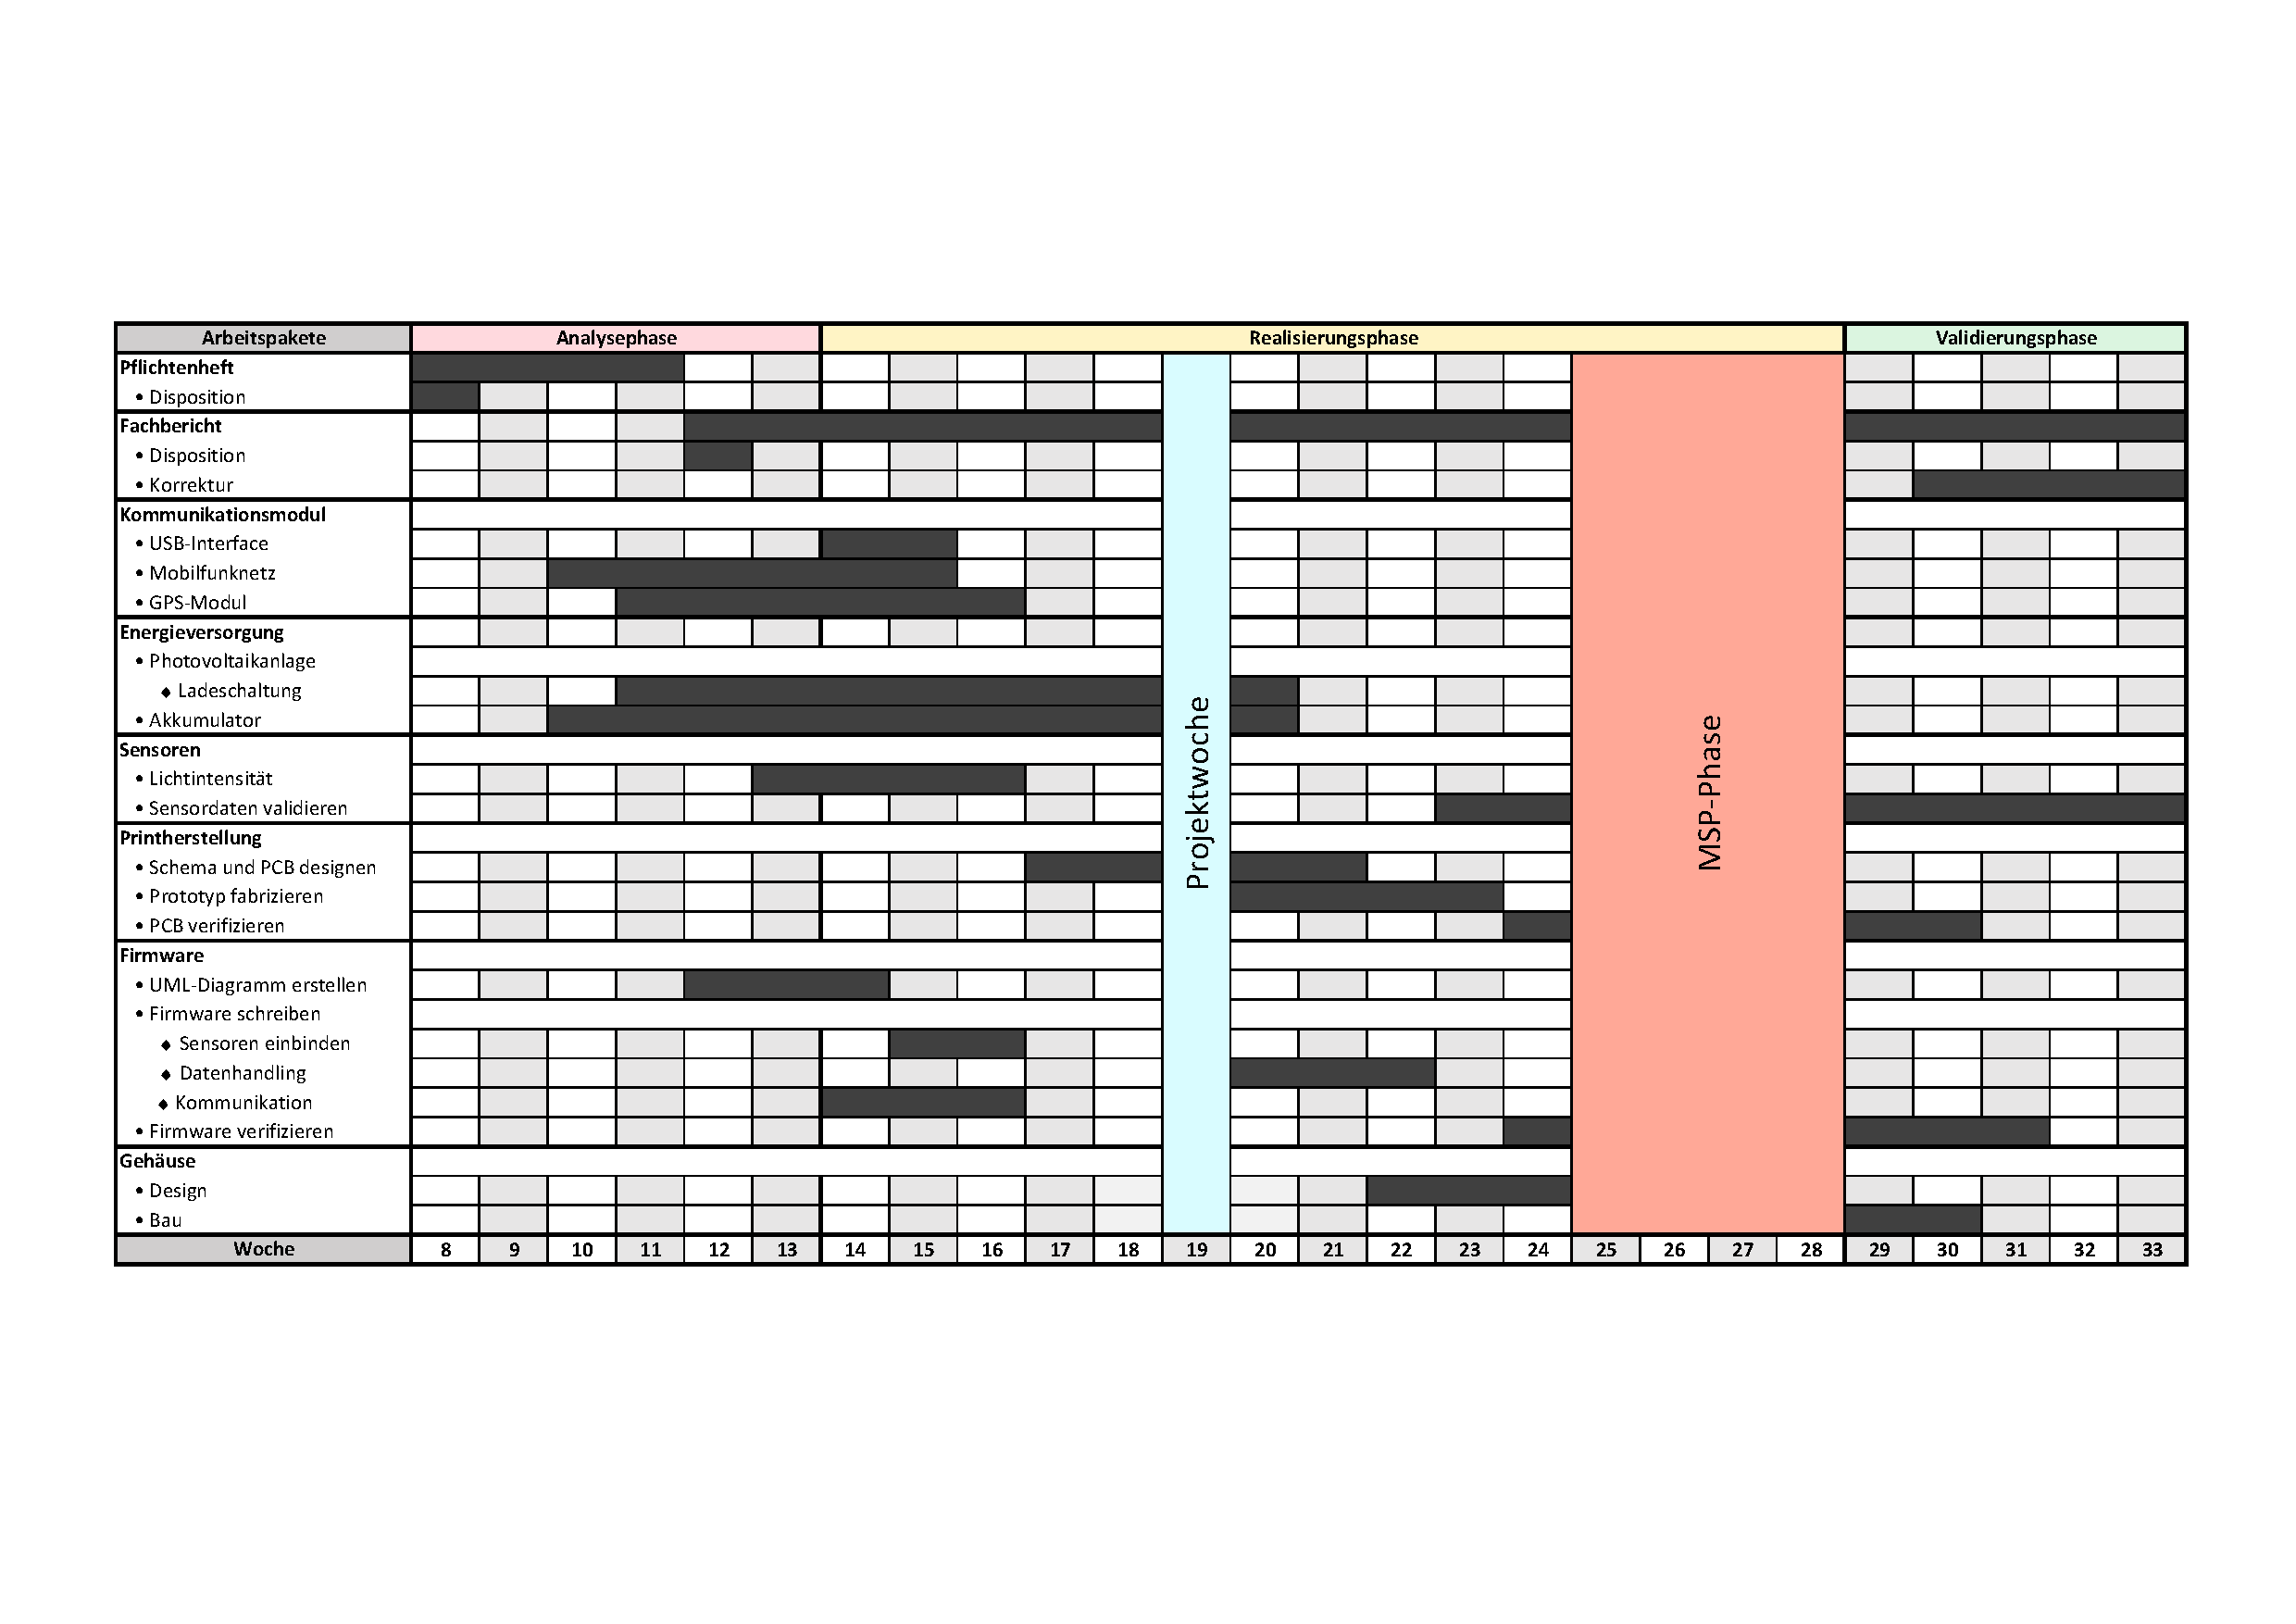
\includepdf[pages={1},nup=1x1,landscape=true,scale=0.85,offset=0 -40,pagecommand={\subsection{Zeitplan Projektverlauf}\label{tab:zeitplan}\thispagestyle{myheadings}}]{graphics/Zeitplanung/prov_zeitplanung.pdf} 
\newpage
\subsection{Einverständniserklärung}
Die unterzeichnenden Projektinstanzen bestätigen hiermit, dass sie dieses Dokument gelesen haben und die Rahmenbedingungen somit
akzeptieren.

%%---BIBLIOGRAPHY------------------------------------------------------------------------
\bibliography{literature/bibliography}

%%---APPENDIX----------------------------------------------------------------------------
\begin{appendix}
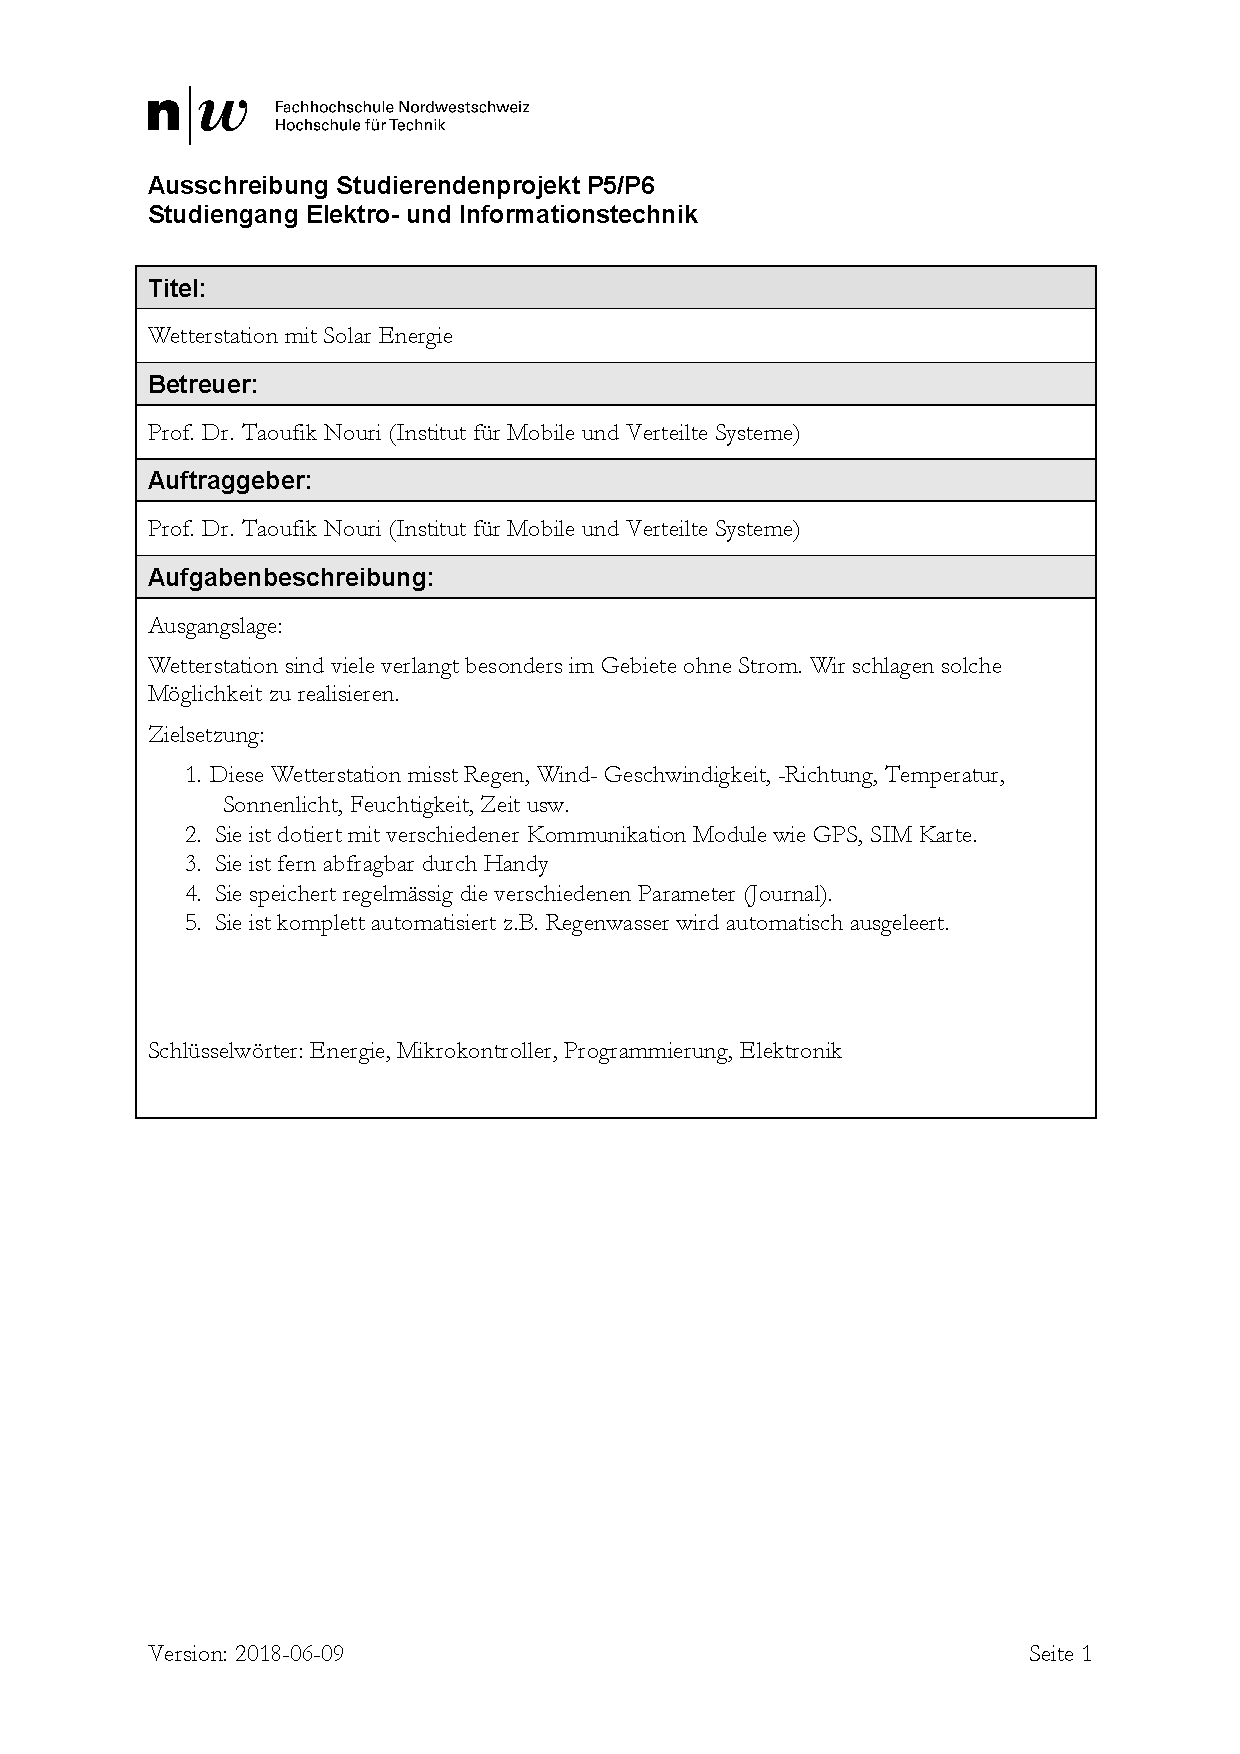
\includepdf[pages={1},nup=1x1,landscape=false,scale=0.85,offset=0 -40,pagecommand={\section{Lastenheft}\label{tab:zeitplan}\thispagestyle{myheadings}}]{appendix/Auftragsbeschreibung.pdf} \newpage
\end{appendix}

%%---NOTES for DEBUG---------------------------------------------------------------------
\ifdraft{%Do this only if mode=draft
%%requires \usepackage{todonotes})
\newpage
\listoftodos[\section{Todo-Notes}]
\clearpage
}
{%Do this only if mode=final
\listoftodos[\section{Todo-Notes}]
}
\end{document}
